% ******************************* PhD Thesis Template **************************
% Please have a look at the README.md file for info on how to use the template

\documentclass[a4paper,12pt,times,numbered,print,index,custommargin]{Classes/PhDThesisPSnPDF}

\usepackage{nomencl} 
\makenomenclature


% `a4paper'(The Politecnico di Torino PhD thesis guidelines recommends a page
% size a4 - default option) or `a5paper'%
% `11pt' or `12pt'(default): Font Size 10pt is NOT recommended by the University
% guidelines
% `oneside' or `twoside'(default): Printing double side (twoside) or single
% side.
% `print': Use `print' for print version with appropriate margins and page
% layout. Leaving the options field blank will activate Online version.

% `abstract': To generate only the title page and abstract page with
% dissertation title and name, to submit to the Student Registry
%
% `chapter`: This option enables only the specified chapter and it's references
%  Useful for review and corrections.
%
% ************************* Custom Page Margins ********************************
%
% custommargin`: Use `custommargin' in options to activate custom page margins,
% which can be defined in the preamble.tex. Custom margin will override
% print/online margin setup.
%
% *********************** Choosing the Fonts in Class Options ******************
%
% `times' : Times font with math support. (The Polito guidelines
% recommend using times)
%
% `fourier': Utopia Font with Fourier Math font (Font has to be installed)
%            It's a free font.
%
% `customfont': Use `customfont' option in the document class and load the
% package in the preamble.tex
%
% default or leave empty: `Latin Modern' font will be loaded.
%
% ********************** Choosing the Bibliography style ***********************
%
% `authoryear': For author-year citation eg., Rossi (2013)
%
% `numbered': (Default Option) For numbered and sorted citation e.g., [1,5,2]
%
% `custombib': Define your own bibliography style in the `preamble.tex' file.
%              `\RequirePackage[square, sort, numbers, authoryear]{natbib}'.
%              This can be also used to load biblatex instead of natbib
%              (See Preamble)
%
% **************************** Choosing the Page Style *************************
%
% `default (leave empty)': For Page Numbers in Header (Left Even, Right Odd) and
% Chapter Name in Header (Right Even) and Section Name (Left Odd). Blank Footer.
%
% `PageStyleI': Chapter Name next & Page Number on Even Side (Left Even).
% Section Name & Page Number in Header on Odd Side (Right Odd). Footer is empty.
%
% `PageStyleII': Chapter Name on Even Side (Left Even) in Header. Section Number
% and Section Name in Header on Odd Side (Right Odd). Page numbering in footer


% ********************************** Preamble **********************************
% Preamble: Contains packages and user-defined commands and settings
% ******************************************************************************
% ****************************** Custom Margin *********************************

%Add `custommargin' in the document class options to use this section
%Set {innerside margin / outerside margin / topmargin / bottom margin}  and
% other page dimensions
\ifsetCustomMargin
  \RequirePackage[left=35mm,right=35mm,top=40mm,bottom=40mm]{geometry}
  \setFancyHdr % To apply fancy header after geometry package is loaded
\fi

% Add spaces between paragraphs
\setlength{\parskip}{0.5em}
% Ragged bottom avoids extra whitespaces between paragraphs
\raggedbottom
% To remove the excess top spacing for enumeration, list and description
%\usepackage{enumitem}
%\setlist[enumerate,itemize,description]{topsep=0em}

% *****************************************************************************
% ******************* Fonts (like different typewriter fonts etc.)*************

% Add `customfont' in the document class option to use this section

\ifsetCustomFont
  % Set your custom font here and use `customfont' in options. Leave empty to
  % load computer modern font (default LaTeX font).
  %\RequirePackage{helvet}

  % For use with XeLaTeX
  %  \setmainfont[
  %    Path              = ./libertine/opentype/,
  %    Extension         = .otf,
  %    UprightFont = LinLibertine_R,
  %    BoldFont = LinLibertine_RZ, % Linux Libertine O Regular Semibold
  %    ItalicFont = LinLibertine_RI,
  %    BoldItalicFont = LinLibertine_RZI, % Linux Libertine O Regular Semibold Italic
  %  ]
  %  {libertine}
  %  % load font from system font
  %  \newfontfamily\libertinesystemfont{Linux Libertine O}
\fi

% *****************************************************************************
% **************************** Custom Packages ********************************

% ************************* Algorithms and Pseudocode **************************

%\usepackage{algpseudocode}


% ********************Captions and Hyperreferencing / URL **********************

% Captions: This makes captions of figures use a small font.
\RequirePackage[small]{caption}

\RequirePackage[labelsep=space,tableposition=top]{caption}
\renewcommand{\figurename}{Fig.} %to support older versions of captions.sty


% *************************** Graphics and figures *****************************

%\usepackage{rotating}
%\usepackage{wrapfig}

% Uncomment the following two lines to force Latex to place the figure.
% Use [H] when including graphics. Note 'H' instead of 'h'
\usepackage{float}
%\restylefloat{figure}

% Subcaption package is also available in the sty folder you can use that by
% uncommenting the following line
% This is for people stuck with older versions of texlive
%\usepackage{sty/caption/subcaption}
\usepackage{subcaption}

% ********************************** Tables ************************************
\usepackage{booktabs} % For professional looking tables
\usepackage{multirow}

%\usepackage{multicol}
%\usepackage{longtable}
%\usepackage{tabularx}


% *********************************** SI Units *********************************
\usepackage{siunitx} % use this package module for SI units


% ******************************* Line Spacing *********************************

% Choose linespacing as appropriate. Default is one-half line spacing as per the
% University guidelines

% \doublespacing
% \onehalfspacing
% \singlespacing


% ************************ Formatting / Footnote *******************************

% Don't break enumeration (etc.) across pages in an ugly manner (default 10000)
%\clubpenalty=500
%\widowpenalty=500

%\usepackage[perpage]{footmisc} %Range of footnote options


% *****************************************************************************
% *************************** Bibliography  and References ********************

%\usepackage{cleveref} %Referencing without need to explicitly state fig /table

% Add `custombib' in the document class option to use this section
\ifuseCustomBib
   \RequirePackage[square, sort, numbers, authoryear]{natbib} % CustomBib

% If you would like to use biblatex for your reference management, as opposed to the default `natbibpackage` pass the option `custombib` in the document class. Comment out the previous line to make sure you don't load the natbib package. Uncomment the following lines and specify the location of references.bib file

%\RequirePackage[backend=biber, style=numeric-comp, citestyle=numeric, sorting=nty, natbib=true]{biblatex}
%\bibliography{References/references} %Location of references.bib only for biblatex

\fi

% changes the default name `Bibliography` -> `References'
\renewcommand{\bibname}{References}


% ******************************************************************************
% ************************* User Defined Commands ******************************
% ******************************************************************************

% *********** To change the name of Table of Contents / LOF and LOT ************

\renewcommand{\contentsname}{Contents}
\renewcommand{\listfigurename}{List of Figures}
\renewcommand{\listtablename}{List of Tables}


% ********************** TOC depth and numbering depth *************************

\setcounter{secnumdepth}{2}
\setcounter{tocdepth}{2}



% ******************************* Nomenclature *********************************

% To change the name of the Nomenclature section, uncomment the following line
%\renewcommand{\nomname}{Symbols}
%\printnomenclature[space] %space can be set as 2em between symbol and description
%\printnomenclature[3em]

% ********************************* Appendix ***********************************

% The default value of both \appendixtocname and \appendixpagename is `Appendices'. These names can all be changed via:

%\renewcommand{\appendixtocname}{List of appendices}
%\renewcommand{\appendixname}{Appndx}


% ************************ Thesis Information & Meta-data **********************
% Thesis title and author information, refernce file for biblatex
% ************************ Thesis Information ***************************

%% Title of the Degree (for example: mechanical engineering, Architecture,...)
\degreetitle{Energy Engineering}

%% Cycle of the phd program
\cycle{$29^{th}$}

%% The title of the thesis
\title{Writing Your Ph.D. Thesis in\\ \LaTeX}
%\texorpdfstring is used for PDF metadata. Usage:
%\texorpdfstring{LaTeX_Version}{PDF Version (non-latex)} eg.,
%\texorpdfstring{$sigma$}{sigma}

%% Subtitle (Optional)
\subtitle{Using the POLITO Template}

%% The full name of the author
\author{Mario Rossi}
\label{author}

%% Supervisor(s) 
%% for multiple supervisors, append each supervisor with the \\ command
\supervisor{Prof. A.B., Supervisor\\
	Prof. C.D., Co-Supervisor}%\\
	%Prof. E.F. ,Co-Supervisor\\
	%Prof. G.H. ,Co-Supervisor}

%% Committee members and their role, seperate the role and university by ,
\committee{Prof. A.B. , Referee, University of...\\
	Prof. C.D, Referee, University of... \\
	Prof. E.F, University of... \\ 
	Prof. G.H, University of... \\ 
	Prof. I.J, University of...}


%% Submission date
% Default is set as {\the\year}. In the case you want to change it use the command:
%\degreedate{2014} 

%% Meta information
\subject{LaTeX} \keywords{{LaTeX} {PhD Thesis} {Engineering} {Politecnico di Torino}}


% ***************************** Abstract Separate ******************************
% To printout only the titlepage and the abstract with the PhD title and the
% author name for submission to the Student Registry, use the `abstract' option in
% the document class.

\ifdefineAbstract
 \pagestyle{empty}
 \includeonly{Declaration/declaration, Abstract/abstract}
\fi

% ***************************** Chapter Mode ***********************************
% The chapter mode allows user to only print particular chapters with references
% Title, Contents, Frontmatter are disabled by default
% Useful option to review a particular chapter or to send it to supervisior.
% To use choose `chapter' option in the document class:

\ifdefineChapter
 \includeonly{Chapter3/chapter3}
\fi
% Then you can select the desired chapter (here is 3) to print.

% ******************************** Front Matter ********************************
\begin{document}

\frontmatter

\maketitle

% ******************************* Thesis Declaration ***************************

\begin{declaration}

I hereby declare that, the contents and organization of this dissertation constitute my own original work and does not compromise in any way the rights of third parties, including those relating to the security of personal data.

% Author and date will be inserted automatically from thesis.tex \author \degreedate

\end{declaration}


% ******************************* Thesis Dedidcation ********************************

\begin{dedication} 

\textit{I would like to dedicate this thesis to my loving parents} 

\end{dedication}


% ************************** Thesis Acknowledgements **************************

\begin{acknowledgements}      


And I would like to acknowledge ...


\end{acknowledgements}

% ************************** Thesis Abstract *****************************
% Use `abstract' as an option in the document class to print only the titlepage and the abstract.
% The maximum number of characters in abstract must be 4000 (defined by PhD school of Politecnico di Torino). 
\begin{abstract}
This is where you write your abstract ... (Max= 4000 characters)
\end{abstract}


% *********************** Adding TOC and List of Figures and tables*************
% By activating (commenting out) these comands the table of contents, list of  
% figures and list of tables auotomatically apear.

\tableofcontents

\listoffigures

\listoftables

% ********************************** Nomenclature ******************************
\printnomenclature


% ******************************** Main Matter *********************************
\mainmatter

%*******************************************************************************
%*********************************** First Chapter *****************************
%*******************************************************************************

\chapter{First Chapter Title}  %Title of the First Chapter
\label{chapter 1}
\ifpdf
    \graphicspath{{Chapter1/Figs/}{Chapter1/Figs/PDF/}{Chapter1/Figs/}}
\else
    \graphicspath{{Chapter1/Figs/Vector/}{Chapter1/Figs/}}
\fi


%********************************** %First Section  ****************************
\section{Introduction to PhD Thesis Template} %Section - 1.1 
\label{section 1.1} % here you can label the section to refer it inside the text

Welcome to this \LaTeX{} Thesis Template for writing your PhD thesis using the \LaTeX{} typesetting system. If you are writing a thesis (or will be in the future) and its subject is technical or mathematical (though it doesn't have to be), then creating it in \LaTeX{} is highly recommended.

\LaTeX{} is easily able to professionally typeset documents that run to hundreds or thousands of pages long. With simple mark-up commands, it automatically sets out the table of contents, margins, page headers and footers and keeps the formatting consistent and beautiful. One of its main strengths is the way it can easily typeset mathematics, even heavy mathematics. Even if those equations are the most horribly twisted and most difficult mathematical problems that can only be solved on a super-computer, you can at least count on \LaTeX{} to make them look stunning \cite{lamport1994latex, hertel2010writing}.Please see appendix\ref{Appendix1} for the instruction to install \LaTeX.

Along with this document you have access to \LaTeX{} file (\textbf{Polito PhD thesis template.tex}) including different partitions: Preamble, Thesis info and etc. Inside each part there are instructive comments explaining the options for different commands. The default commands are designed and recommended by PhD school of Politecnico di Torino. In this tutorial the commands essential to write a scientific document are listed and explained briefly.  




%********************************** %Second Section  ***************************
\section{Getting Started with this Template}  %Section - 1.2 
\label{section1.2}
If you are familiar with \LaTeX{}, then you should explore the directory structure of the template and then proceed to place your own information into the  block of the \textbf{Polito PhD thesis template.tex} file. You can then modify the rest of this file to your unique specifications based on your course. Chapter \ref{chapter 2} will help you do this.

If you are new to \LaTeX{} it is recommended that you carry on reading through the rest of the information in this document. The style of this template is confirmed and recommanded by Doctoral School of Politecnico di Torino (SCUDO).

%********************************** % Third Section  ***************************
\section{What this Template Includes}
\label{section 1.3}

\subsection{Folders}

This template comes as a single zip file that expands out to several files and folders. The folder names are mostly self-explanatory:

\textbf{Preamble}: this folder contains the \textbf{.tex} file in which the adjustments and modifications regarding the style of document is possible. It is recommanded to not changing the predefined style, except for small modifications.

\textbf{Thesis-info}: this folder contains the \textbf{.tex} file in which the thesis informations can be inserted.
 
\textbf{Dedication}: this folder contains the \textbf{.tex} file dedicated to write the dedications of the thesis.

\textbf{Declaration}: this folder contains the \textbf{.tex} file dedicated to write the declaration of the thesis.

\textbf{Acknowledgment}: this folder contains the \textbf{.tex} file dedicated to write the acknowledgments of the thesis. 

\textbf{Abstract}: this folder contains the \textbf{.tex} file dedicated to write the abstract of the thesis.

\textbf{Chapters}: these are the folders where you put the thesis chapters.  Each chapter should go in its own separate \textbf{.tex} file and folder. Each chapter folder contains a \textbf{Figs} folder which contains all figures for the chapter. A thesis usually has about five to six chapters, though there is no hard rule on this. For example they can be split as:
\begin{itemize}
	\item Chapter 1: Introduction to the thesis topic
	\item Chapter 2: Background information and theory
	\item Chapter 3: (Laboratory) experimental setup
	\item Chapter 4: Details of experiment
	\item Chapter 5: Discussion of the experimental results
	\item Chapter 6: Conclusion and future directions
\end{itemize}
This chapter layout is specialised for the experimental sciences.

\textbf{Figs}: This folder contains all figures for the thesis not included in chapters (for exaple the polito logo on thesis info page). These are the final images that will go into the thesis document.

\textbf{References}: this folder contains the \textbf{.tex} file which is an important file that contains all the bibliographic information and references that you will be citing in the thesis for use with BibTeX. You can write it manually, but there are reference manager programs available that will create and manage it for you. Bibliographies in \LaTeX{} are a large subject and you may need to read about BibTeX before starting with this. Many modern reference managers will allow you to export your references in BibTeX format which greatly eases the amount of work you have to do..

\textbf{Classes} and \textbf{sty}: these folders contain important files such as class file that tells \LaTeX{} how to format the thesis.

\textbf{Appendices}: these are the folders where you put the appendices. Each appendix should go into its own separate \textbf{.tex} file.

\subsection{Files}

Included are also several files, most of them are plain text and you can see their contents in a text editor. After initial compilation, you will see that more auxiliary files are created by \LaTeX{} or BibTeX and which you don't need to delete or worry about:

\textbf{Polito PhD thesis template.pdf}: this is your beautifully typeset thesis (in the PDF file format) created by \LaTeX{}. It is supplied in the PDF with the template and after you compile the template you should get an identical version.

\textbf{Polito PhD thesis template.tex}: this is an important file. This is the file that you tell \LaTeX{} to compile to produce your thesis as a PDF file. It contains the framework and constructs that tell \LaTeX{} how to layout the thesis. It is heavily commented so you can read exactly what each line of code does and why it is there. After you put your own information into the \emph{Thesis-info} block -- you have now started your thesis!

Files that are \emph{not} included, but are created by \LaTeX{} as auxiliary files include:\textbf{.aux}, \textbf{.bbl}, \textbf{.blg}, \textbf{.lof}, \textbf{.log}, \textbf{.lot} and \textbf{.out} files: are auxiliary files generated by \LaTeX{}, if they are deleted \LaTeX{} simply regenerates them when you run the main \textbf{.tex} file.

%********************************** % Forth Section  ****************************

\section{Filling in Your Information in the "Polito PhD thesis template.tex" File}
\label{section 1.4}

You will need to personalise the thesis template and make it your own by filling in your own information. This is done by editing the \textbf{Polito PhD thesis template.tex} file in a text editor or your favourite LaTeX environment.

Open the file and scroll down to the second large block titled \emph{Thesis-info} where you can see the entries for \emph{Authur}, \emph{Supervisors}, etc \ldots. Fill out the information about your thesis, yourself and your department. When you have done this, save the file and recompile \textbf{Polito PhD thesis template.tex}. All the information you filled in should now be in the PDF, complete with web links. You can now begin your thesis proper!

The \textbf{Polito PhD thesis template.tex} file contains the structure of the thesis. There are plenty of written comments that explain what pages, sections and formatting the \LaTeX{} code is creating. Each major document element is divided into commented blocks with titles in all capitals to make it obvious what the following bit of code is doing. Initially there seems to be a lot of \LaTeX{} code, but this is all formatting, and it has all been taken care of so you don't have to do it.

Begin by checking that your information on the title page is correct. The next page contains a one line (or more) dedication; Who will you dedicate your thesis to. Next come the acknowledgements. On this page, write about all the people who you wish to thank (not forgetting parents, partners and your advisor/supervisor).Following this is the abstract page which summarises your work in a condensed way and can almost be used as a standalone document to describe what you have done. The text you write will cause the heading to move up so don't worry about running out of space.

The contents pages, list of figures and tables are all taken care of for you and do not need to be manually created or edited.  Finally, there is the block where the chapters are included. Uncomment the lines (delete the \% character) as you write the chapters. Each chapter should be written in its own file and put into the \emph{Chapters} folder and named Chapter1, Chapter2, etc\ldots Similarly for the appendices, uncomment the lines as you need them. Each appendix should go into its own file and placed in the Appendices folder.

After the preamble, chapters and appendices finally comes the bibliography. The bibliography style (called \textbf{numbered}) is used for the bibliography and is a fully featured style that will even include links to where the referenced paper can be found online. Do not underestimate how grateful your reader will be to find that a reference to a paper is just a click away. Of course, this relies on you putting the URL information into the BibTeX file in the first place.
%*******************************************************************************
%****************************** Second Chapter *********************************
%*******************************************************************************

\chapter{Second Chapter Title}
\label{chapter 2}
\ifpdf
    \graphicspath{{Chapter2/Figs/}{Chapter2/Figs/PDF/}{Chapter2/Figs/}}
\else
    \graphicspath{{Chapter2/Figs/Vector/}{Chapter2/Figs/}}
\fi
%********************************** % First Section  *************************************
\section{Basic Text and Refering Hints}
\LaTeX gives the possibility to bold a \textbf{word} or a \textbf{phrase containing more words} or mathematical equations like $\mathbf{A=B+C}$. \textit{Italic} and \underline{underline} commands are designed to be used in desired partof the text. Sizing the text is another optional command:
{\small Word}, {\large Word}, {\Large Word}.

%other options:
% \Huge
% \huge
% \LARGE
% \Large
% \large
% \normalsize (default)
% \small
% \footnotesize
% \scriptsize
% \tiny

Refering to the sections, chapters, equations and etc \dots is possible by command \verb|\ref{label}|. It is necessary to insert \verb|\label{name of section}| for each of desired section and chapter and etc \dots then refer them in any part of the text. For example in chapter \ref{chapter 1} we introduced the template and in section \ref{section 1.3} different folders and files in template were discribed. Figure \ref{fig:Greek} shows the greek letter codes in \LaTeX. 

Moreover in \LaTeX \footnote{Here there is the foot note explanation about the word \LaTeX} it is possible to have foot note explanation. You can also insert web links, if you do, make sure you use the full URL, including the \{http://\} for this. As an example by inserting the code: \begin{verbatim}
\href{http://www.polito.it}{polito website} \end{verbatim} you will have \href{http://www.polito.it}{polito website}. If you don't want to link URL and name, simply write the \verb|\url{http://www.polito.it}| and only romove the name. This is the result: (\url{http://www.polito.it}).

%********************************** % Second Section  *************************************
\section{Writing Mathematical Equations in \LaTeX} %Section - 2.2
\label{section 2.2}
% Uncomment this line, when you have siunitx package loaded.
%The SI Units for dynamic viscosity is \si{\newton\second\per\metre\squared}.
As an in-line equation example we can refer the most famous equation in the world: $E^2 = (m_0c^2)^2 + (pc)^2$, which is known as the \textbf{energy-mass-momentum} relation. You can write an equation in \textbf{equation} environment of \LaTeX, for example "Cauchy's Integral Formula" which is automatically given an equation number (tag) by \LaTeX{} like this:
\begin{verbatim}
\begin{equation}
CIF: \hspace*{5mm}F_0^j(a) =\frac{1}{2\pi \iota} \oint_{\gamma} 
\frac{F_0^j(z)}{z - a} dz
\end{equation}
\end{verbatim}
This will produce "Cauchy's Integral Formula" equation:

\begin{equation}
CIF: \hspace*{5mm}F_0^j(a) = \frac{1}{2\pi \iota} \oint_{\gamma} \frac{F_0^j(z)}{z - a} dz
\end{equation}

As you see the equation is tagged automatically according to the chapter and order. It is also possible to personalize tag for the equation:
\begin{equation}
\centering
\tag{Personalized tag}
CIF: \hspace*{5mm}F_0^j(a) = \frac{1}{2\pi \iota} \oint_{\gamma} \frac{F_0^j(z)}{z - a} dz
\end{equation}

\nomenclature[Z]{$CIF$}{Cauchy's Integral Formula}                                
% letter Z is for Acronyms 
\nomenclature[A]{$F$}{complex function}                                                  
%  letter A is for Roman symbols
\nomenclature[G]{$\pi$}{ $\simeq 3.14\ldots$}                                             
% letter G is for Greek Symbols
\nomenclature[G]{$\iota$}{unit imaginary number $\sqrt{-1}$}                      
% first letter G is for Greek Symbols
\nomenclature[G]{$\gamma$}{a simply closed curve on a complex plane}  
% first letter G is for Greek Symbols
\nomenclature[X]{$\oint_\gamma$}{integration around a curve $\gamma$} 
% first letter X is for Other Symbols
\nomenclature[R]{$j$}{superscript index}                                                       
% first letter R is for superscripts
\nomenclature[S]{$0$}{subscript index}
% first letter S is for subscripts

To make the \textbf{Nomenculature } you need to Issue the \verb|\nomenclature| command for each symbol you want to have included in the nomenclature list. The best place for this command is immediately after you introduce the symbol for
the first time. For the equation above:

\begin{verbatim}
\nomenclature[Z]{$CIF$}{Cauchy's Integral Formula}                                
\nomenclature[A]{$F$}{complex function}                                                  
\nomenclature[G]{$\pi$}{ $\simeq 3.14\ldots$}                                             
\nomenclature[G]{$\iota$}{unit imaginary number $\sqrt{-1}$}                      
\nomenclature[G]{$\gamma$}{a closed curve on a complex plane}  
\nomenclature[X]{$\oint_\gamma$}{integration around a curve 
$\gamma$} 
\nomenclature[R]{$j$}{superscript index}                                                       
\nomenclature[S]{$0$}{subscript index}
%letter Z is for Acronyms, A is for Roman symbols, G is for Greek 
Symbols, X is for Other Symbols letter, R is for superscripts, S 
is for subscripts
\end{verbatim}

To make nomenclature list you need to run "pdflatex" for \textbf{.tex} file and then run the "makeindex" command and then again run "pdflatex" for \textbf{.tex} file. (make sure in "Options> Configurations >Commands >make index" box there is "makeindex -s nomencl.ist -t \%.nlg -o \%.nls \%.nlo", if not, just copy and paste this command in the box and follow the instruction above).


If there are several equations that you need to align vertically, the \textbf{align} environment will do it:
\begin{align*}
	x&=5y           &  w &=-z              &  a&=b-c\\
	2x&=-y         &  3w&=\frac{1}{2}z   &  a&=3b\\
	-4 + 5x&=2+y   &  w+2&=-1+w          &  ab&=\frac{-1}{3}cb
\end{align*}

%using * will remove the tags from equations.

\vspace{0.5cm}

%********************************** % Third Section  ***************************
\section{List Formatting in \LaTeX}
\label{section 2.3}
Convenient and predictable list formatting is one of the many advantages of using \LaTeX . Latex distinguishes between three different enumeration/itemization environments: 
%
\begin{itemize}
	\item Enumerate for an enumerated list,
	\item Itemize for a bullet list,
	\item Description for a descriptive list.
\end{itemize}
All lists follow a basic format and each of them provide four levels, which means you can have nested lists of up to four levels.

\subsection{Enumerate}

\begin{enumerate}
	\item The first topic is "Good"
	\item The second topic is "Intermediate" (Lev. 1)
	\begin{enumerate}
		\item The first subtopic is "high intermediate"
		\item The second subtopic is "low intermediate"(Lev. 2)
		\begin{enumerate}
			\item The first subsubtopic is "very low intermediate"(Lev. 3)
			\begin{enumerate}
				\item The first subsubsubtopic is "too low intermediate"(Lev. 4)
			\end{enumerate}
		\end{enumerate}
	\end{enumerate}
	\item The third topic is "Bad"
\end{enumerate}
 

\subsection{Itemize}

\begin{itemize}
	\item The first topic is "Good"
    \item The second topic is "Intermediate"
    \begin{itemize}
	     \item The first subtopic is "high intermediate"
	     \item The second subtopic is "low intermediate"
	     \begin{itemize}
		      \item The first subsubtopic is "very low intermediate"
	     \end{itemize}
\end{itemize}
\item The third topic is "Bad"
\end{itemize}

\subsection{Description}
\begin{description}
	\item [The first topic] is "Good"
    \item [The second topic] is "Intermediate"
    \begin{description}
	      \item [The first subtopic] is "high intermediate"
	      \item [The second subtopic] is "low intermediate"
	      \begin{description}
		        \item [The first subsubtopic] is "very low intermediate"
	      \end{description}
\end{description}
\item [The third topic] is "Bad"
\end{description}


%********************************** % Forth Section  ***************************

\section{Figures}
\label{section 2.4}
There will hopefully be many figures in your thesis (that should be placed in the \textbf{Figs} folder in each chapter folder). The way to insert figures into your thesis is to use a code template like this:
\begin{verbatim}
\begin{figure}[H] 
\centering    
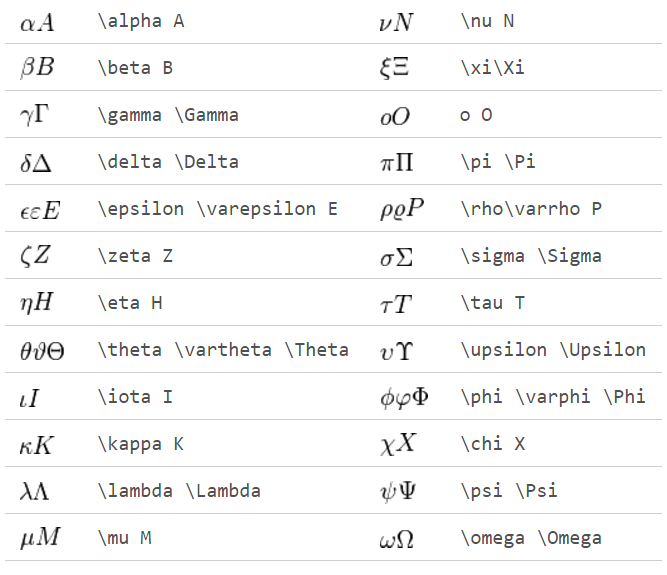
\includegraphics[width=1.0\textwidth]{Greek_letters}
\caption[Greek letters in latex]{List of greek letters in Latex}
\label{fig:Greek}
\end{figure}
\end{verbatim}
Also look in the source file. Putting this code into the source file produces the Figure~\ref{fig:Greek} that you can see in the figure below. By changing the value of figure width (\verb|width=1.0\textwidth|) you can change the figure dimension.

\begin{figure}[H] 
\centering    
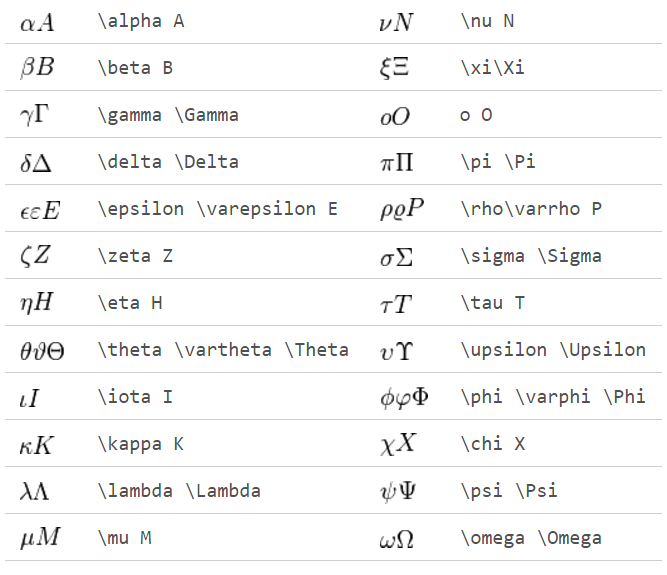
\includegraphics[width=0.8\textwidth]{Greek_letters}
\caption[Greek letters in latex]{List of greek letters in Latex}
\label{fig:Greek}
\end{figure}


\begin{landscape}

\section*{Subplots}
The multiple figure example in landscape form is presented here. Here you can refer any subfigure for example  arrows (see Fig.~\ref{fig:Arrows}) and binary operation symbols in (Fig.~\ref{fig:Miscsymb}) or you can cite the whole figure as Fig.~\ref{fig:Mathsymb}


\begin{figure}
  \centering
  \begin{subfigure}[b]{0.5\textwidth}
    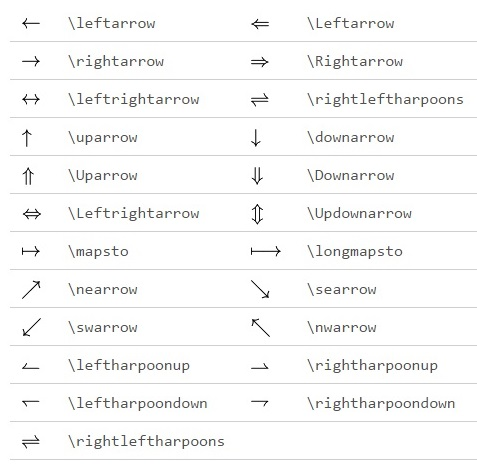
\includegraphics[width=\textwidth]{Arrows}
    \caption{Arrows}
    \label{fig:Arrows}   
  \end{subfigure}             
  \begin{subfigure}[b]{0.5\textwidth}
    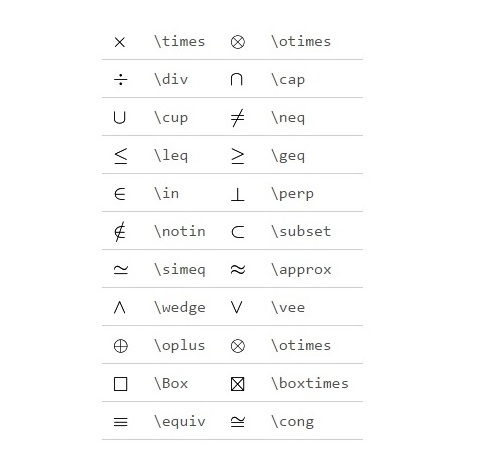
\includegraphics[width=\textwidth]{Binary_operations}
    \caption{Binary operations symbols}
    \label{fig:Binarysymb}
  \end{subfigure}             
  \begin{subfigure}[b]{0.5\textwidth}
    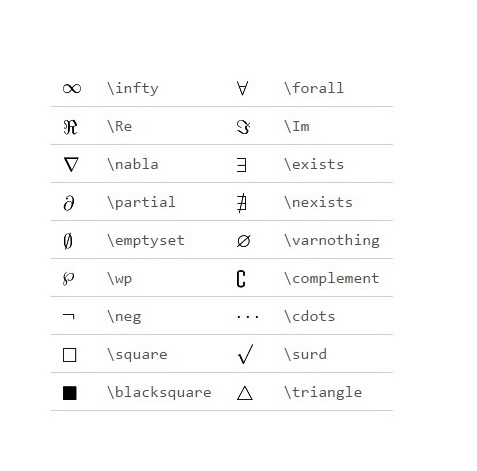
\includegraphics[width=\textwidth]{Miscellaneous_symbols}
    \caption{Miscellaneous sybols}
    \label{fig:Miscsymb}
  \end{subfigure}
  \caption{Useful math symbols in Latex}
  \label{fig:Mathsymb}
\end{figure}

\end{landscape}

%********************************** % Fifth Section  ***************************
\section{Tables}

The layout of a table has been established over centuries of experience and 
should only be altered in extraordinary circumstances \cite{fear2005publication}. 

When formatting a table, remember two simple guidelines at all times:

\begin{enumerate}
	\item Never, ever use vertical rules (lines).
	\item Never use double rules.
\end{enumerate}

These guidelines may seem extreme but I have
never found a good argument in favour of breaking them. For
example, if you feel that the information in the left half of
a table is so different from that on the right that it needs
to be separated by a vertical line, then you should use two
tables instead. Not everyone follows the second guideline:

There are three further guidelines worth mentioning here as they
are generally not known outside the circle of professional
typesetters and subeditors:
\begin{enumerate}\setcounter{enumi}{2}
	\item Put the units in the column heading (not in the body of
	the table).
	\item Always precede a decimal point by a digit; thus 0.1
	{\em not} just .1.
	\item Do not use `ditto' signs or any other such convention to
	repeat a previous value. In many circumstances a blank
	will serve just as well. If it won't, then repeat the value.
\end{enumerate}
A frequently seen mistake is to use `\textbackslash begin\{center\}' \dots `\textbackslash end\{center\}' inside a figure or table environment. This center environment can cause additional vertical space. If you want to avoid that just use `\textbackslash centering'

\begin{table}
	\caption{A badly formatted table}
	\centering
	\label{table:bad_table}
	\begin{tabular}{|l|c|c|c|c|}
		\hline 
		& \multicolumn{2}{c}{Species I} & \multicolumn{2}{c|}{Species II} \\ 
		\hline
		Dental measurement  & mean & SD  & mean & SD  \\ \hline 
		\hline
		I1MD & 6.23 & 0.91 & 5.2  & 0.7  \\
		\hline 
		I1LL & 7.48 & 0.56 & 8.7  & 0.71 \\
		\hline 
		I2MD & 3.99 & 0.63 & 4.22 & 0.54 \\
		\hline 
		I2LL & 6.81 & 0.02 & 6.66 & 0.01 \\
		\hline 
		CMD & 13.47 & 0.09 & 10.55 & 0.05 \\
		\hline 
		CBL & 11.88 & 0.05 & 13.11 & 0.04\\ 
		\hline 
	\end{tabular}
\end{table}

\begin{table}
	\caption{A nice looking table}
	\centering
	\label{table:nice_table}
	\begin{tabular}{l c c c c}
		\hline 
		\multirow{2}{*}{Dental measurement} & \multicolumn{2}{c}{Species I} & \multicolumn{2}{c}{Species II} \\ 
		\cline{2-5}
		& mean & SD  & mean & SD  \\ 
		\hline
		I1MD & 6.23 & 0.91 & 5.2  & 0.7  \\
		
		I1LL & 7.48 & 0.56 & 8.7  & 0.71 \\
		
		I2MD & 3.99 & 0.63 & 4.22 & 0.54 \\
		
		I2LL & 6.81 & 0.02 & 6.66 & 0.01 \\
		
		CMD & 13.47 & 0.09 & 10.55 & 0.05 \\
		
		CBL & 11.88 & 0.05 & 13.11 & 0.04\\ 
		\hline 
	\end{tabular}
\end{table}


\begin{table}
	\caption{Even better looking table using booktabs}
	\centering
	\label{table:good_table}
	\begin{tabular}{l c c c c}
		\toprule
		\multirow{2}{*}{Dental measurement} & \multicolumn{2}{c}{Species I} & \multicolumn{2}{c}{Species II} \\ 
		\cmidrule{2-5}
		& mean & SD  & mean & SD  \\ 
		\midrule
		I1MD & 6.23 & 0.91 & 5.2  & 0.7  \\
		
		I1LL & 7.48 & 0.56 & 8.7  & 0.71 \\
		
		I2MD & 3.99 & 0.63 & 4.22 & 0.54 \\
		
		I2LL & 6.81 & 0.02 & 6.66 & 0.01 \\
		
		CMD & 13.47 & 0.09 & 10.55 & 0.05 \\
		
		CBL & 11.88 & 0.05 & 13.11 & 0.04\\ 
		\bottomrule
	\end{tabular}
\end{table}

\chapter{My third chapter}

% **************************** Define Graphics Path **************************
\ifpdf
    \graphicspath{{Chapter3/Figs/}{Chapter3/Figs/PDF/}{Chapter3/Figs/}}
\else
    \graphicspath{{Chapter3/Figs/Vector/}{Chapter3/Figs/}}
\fi
You should break your thesis up into nice, bite-sized sections and subsections. \LaTeX{} automatically builds a table of Contents by looking at all the \verb|\chapter{}|, \verb|\section{}|  and \verb|\subsection{}| commands you write in the source.

The Table of Contents should only list the sections to three (3) levels. A \verb|chapter{}| is level zero (0). A \verb|\section{}| is level one (1) and so a \verb|\subsection{}| is level two (2). In your thesis it is likely that you will even use a \verb|subsubsection{}|, which is level three (3). The depth to which the Table of Contents is formatted is set within \textbf{PhDThesisPSnPDF.cls}. If you need this changed, you can do it in \textbf{Polito PhD thesis template.tex}. 

\section{First section of the third chapter}
And now I begin my third chapter here \dots


\subsection{First subsection in the first section}
\dots and some more 

\subsection{Second subsection in the first section}
\dots and some more \dots

\subsubsection{First subsub section in the second subsection}
\dots and some more in the first subsub section otherwise it all looks the same
doesn't it? well we can add some text to it \dots

\subsection{Third subsection in the first section}
\dots and some more \dots

\subsubsection{First subsub section in the third subsection}
\dots and some more in the first subsub section otherwise it all looks the same
doesn't it? well we can add some text to it and some more \dots

\subsubsection{Second subsub section in the third subsection}
\dots and some more in the second subsub section otherwise it all looks the same
doesn't it? well we can add some text to it \dots

\section{Second section of the third chapter}
and here I write more \dots

\section{In Closing}

You have reached the end of this mini-guide. You can now rename or overwrite this pdf file and begin writing the rest of your thesis. The easy work of setting up the structure and framework has been taken care of for you. It's now your job to fill it out!

Good luck and have fun!


%\include{Chapter4/chapter4}
%\include{Chapter5/chapter5}
%\include{Chapter6/chapter6}
%\include{Chapter7/chapter7}



% ********************************** Back Matter *******************************
% Backmatter should be commented out, if you are using appendices after References
%\backmatter

% ********************************** Bibliography ******************************
\begin{spacing}{0.9}

% To use the conventional natbib style referencing
% Bibliography style previews: http://nodonn.tipido.net/bibstyle.php
% Reference styles: http://sites.stat.psu.edu/~surajit/present/bib.htm

%\bibliographystyle{apalike}
\bibliographystyle{unsrt} % Use for unsorted references  
%\bibliographystyle{plainnat} % use this to have URLs listed in References
\cleardoublepage
\bibliography{References/references} % Path to your References.bib file


% If you would like to use BibLaTeX for your references, pass `custombib' as
% an option in the document class. The location of 'reference.bib' should be
% specified in the preamble.tex file in the custombib section.
% Comment out the lines related to natbib above and uncomment the following line.

%\printbibliography[heading=bibintoc, title={References}]


\end{spacing}

% ********************************** Appendices ********************************

\begin{appendices} % Using appendices environment for more functunality

% ******************************* Thesis Appendix A ****************************
\chapter{How to install \LaTeX} 
\label{Appendix1}
\section*{Windows OS}

\subsection*{TeXLive package - full version}
\begin{enumerate}
\item	Download the TeXLive ISO (2.2GB) from\\
\href{https://www.tug.org/texlive/}{https://www.tug.org/texlive/}
\item	Download WinCDEmu (if you don't have a virtual drive) from \\
\href{http://wincdemu.sysprogs.org/download/}
{http://wincdemu.sysprogs.org/download/}
\item	To install Windows CD Emulator follow the instructions at\\
\href{http://wincdemu.sysprogs.org/tutorials/install/}
{http://wincdemu.sysprogs.org/tutorials/install/}
\item	Right click the iso and mount it using the WinCDEmu as shown in \\
\href{http://wincdemu.sysprogs.org/tutorials/mount/}{
http://wincdemu.sysprogs.org/tutorials/mount/}
\item	Open your virtual drive and run setup.pl
\end{enumerate}

or

\subsection*{Basic MikTeX - \TeX~ distribution}
\begin{enumerate}
\item	Download Basic-MiK\TeX (32bit or 64bit) from\\
\href{http://miktex.org/download}{http://miktex.org/download}
\item	Run the installer 
\item	To add a new package go to Start >> All Programs >> MikTex >> Maintenance (Admin) and choose Package Manager
\item	Select or search for packages to install
\end{enumerate}

\subsection*{TexStudio - \TeX~ editor}
\begin{enumerate}
\item	Download TexStudio from\\
\href{http://texstudio.sourceforge.net/\#downloads}
{http://texstudio.sourceforge.net/\#downloads} 
\item	Run the installer
\end{enumerate}

\section*{Mac OS X}
\subsection*{MacTeX - \TeX~ distribution}
\begin{enumerate}
\item	Download the file from\\
\href{https://www.tug.org/mactex/}{https://www.tug.org/mactex/}
\item	Extract and double click to run the installer. It does the entire configuration, sit back and relax.
\end{enumerate}

\subsection*{TexStudio - \TeX~ editor}
\begin{enumerate}
\item	Download TexStudio from\\
\href{http://texstudio.sourceforge.net/\#downloads}
{http://texstudio.sourceforge.net/\#downloads} 
\item	Extract and Start
\end{enumerate}


\section*{Unix/Linux}
\subsection*{TeXLive - \TeX~ distribution}
\subsubsection*{Getting the distribution:}
\begin{enumerate}
\item	TexLive can be downloaded from\\
\href{http://www.tug.org/texlive/acquire-netinstall.html}
{http://www.tug.org/texlive/acquire-netinstall.html}.
\item	TexLive is provided by most operating system you can use (rpm,apt-get or yum) to get TexLive distributions
\end{enumerate}

\subsubsection*{Installation}
\begin{enumerate}
\item	Mount the ISO file in the mnt directory
\begin{verbatim}
mount -t iso9660 -o ro,loop,noauto /your/texlive####.iso /mnt
\end{verbatim}

\item	Install wget on your OS (use rpm, apt-get or yum install)
\item	Run the installer script install-tl.
\begin{verbatim}
	cd /your/download/directory
	./install-tl
\end{verbatim}
\item	Enter command `i' for installation

\item	Post-Installation configuration:\\
\href{http://www.tug.org/texlive/doc/texlive-en/texlive-en.html\#x1-320003.4.1}
{http://www.tug.org/texlive/doc/texlive-en/texlive-en.html\#x1-320003.4.1} 
\item	Set the path for the directory of TexLive binaries in your .bashrc file
\end{enumerate}

\subsubsection*{For 32bit OS}
For Bourne-compatible shells such as bash, and using Intel x86 GNU/Linux and a default directory setup as an example, the file to edit might be \begin{verbatim}
edit $~/.bashrc file and add following lines
PATH=/usr/local/texlive/2011/bin/i386-linux:$PATH; 
export PATH 
MANPATH=/usr/local/texlive/2011/texmf/doc/man:$MANPATH;
export MANPATH 
INFOPATH=/usr/local/texlive/2011/texmf/doc/info:$INFOPATH;
export INFOPATH
\end{verbatim}
\subsubsection*{For 64bit OS}
\begin{verbatim}
edit $~/.bashrc file and add following lines
PATH=/usr/local/texlive/2011/bin/x86_64-linux:$PATH;
export PATH 
MANPATH=/usr/local/texlive/2011/texmf/doc/man:$MANPATH;
export MANPATH 
INFOPATH=/usr/local/texlive/2011/texmf/doc/info:$INFOPATH;
export INFOPATH

\end{verbatim}



%\subsection{Installing directly using Linux packages} 
\subsubsection*{Fedora/RedHat/CentOS:}
\begin{verbatim} 
sudo yum install texlive 
sudo yum install psutils 
\end{verbatim}


\subsubsection*{SUSE:}
\begin{verbatim}
sudo zypper install texlive
\end{verbatim}


\subsubsection*{Debian/Ubuntu:}
\begin{verbatim} 
sudo apt-get install texlive texlive-latex-extra 
sudo apt-get install psutils
\end{verbatim}

%% ******************************* Thesis Appendix B ********************************

\chapter{title of appendix}





\end{appendices}


% *************************************** Index ********************************
\printthesisindex % If index is present

\end{document}
